\newcommand{\ein}[2]{(#1) (#2 Punkte)}
\newcommand{\frage}[2]{Frage #1 (#2 Punkte)}

\begin{Large}
\textbf{Teil I: Offene Aufgaben (50 Punkte)}
\end{Large}
\\
\\
\\
\textbf{Allgemeine Anweisungen für offene Fragen:}
\\
\renewcommand{\labelenumi}{(\roman{enumi})}
\begin{enumerate}
\item
Ihre Antworten müssen alle Rechenschritte enthalten,
diese müssen klar ersichtlich sein.
Verwendung korrekter mathematischer Notation wird erwartet
und fliesst in die Bewertung ein.

\item
Ihre Antworten zu den jeweiligen Teilaufgaben müssen in den dafür vorgesehenen Platz geschrie-
ben werden. Sollte dieser Platz nicht ausreichen, setzen Sie Ihre Antwort auf der Rückseite oder
dem separat zur Verfügung gestellten Papier fort. Verweisen Sie in solchen Fällen ausdrücklich
auf Ihre Fortsetzung. Bitte schreiben Sie zudem Ihren Vor- und Nachnamen auf jeden separaten
Lösungsbogen.

\item
Es werden nur Antworten im dafür vorgesehenen Platz bewertet. Antworten auf der Rückseite
oder separatem Papier werden nur bei einem vorhandenen und klaren Verweis darauf bewertet.

\item
Die Teilaufgaben werden mit den jeweils oben auf der Seite angegebenen Punkten bewertet.

\item
Ihre endgültige Lösung jeder Teilaufgabe darf nur eine einzige Version enthalten.

\item
Zwischenrechnungen und Notizen müssen auf einem getrennten Blatt gemacht werden. Diese
Blätter müssen, deutlich als Entwurf gekennzeichnet, ebenfalls abgegeben werden.
\end{enumerate}

\newpage
\section*{\hfil Aufgaben \hfil}
\vspace{1cm}
\section*{Aufgabe 1 (26 Punkte)}
\vspace{0.4cm}
\subsection*{(a) (5 Punkte)}
Sei $q(x) = \frac{5x+2}{3x-10}$ für $x \in \mathbb{R} \setminus \left\lbrace \frac{10}{3} \right\rbrace$.
\\
\\
Für welche Werte von $x$ konvergiert die Reihe $\lbrace s_n \rbrace_{n \in \mathbb{N}}$
mit $s_n = \sum_{k=0}^{n-1} 3 \cdot q(x)^k$?
\\
\\
\subsection*{(b) (7 Punkte)} 
Eine Kreditnehmerin leiht sich $P=2'500'000$ CHF, um ihr Haus zu finanzieren.
Sie kann jährliche Zahlungen in Höhe von $C=50'000$ CHF aufbringen.
Der jährliche Zinssatz liegt bei $i = 1 \%$. Wie lange benötigt die Kundin, um das Darlehen zurückzuzahlen, wenn die Zahlungen zum Ende des Jahres stattfinden? 
\\
\\
\subsection*{(c) (5 Punkte)}
Berechnen Sie 
\begin{align*}
\lim \limits_{x \rightarrow \infty} \left(\frac{x+3}{x+2}\right)^{3x+6}.
\end{align*}
\\

\subsection*{(d1) (5 Punkte)}
Gegeben sei die Funktion
\begin{align*}
f \ : \ D_f \to \mathbb{R}, \ \ x \mapsto y = \sqrt{\ln(x^2+4x+4)}.
\end{align*}
Bestimmen Sie den Definitionsbereich $D_f$.
\\
\\
\subsection*{(d2) (4 Punkte)}
Gegeben sei die Funktion
\begin{align*}
f \ : \ D_f \to \mathbb{R}, \ x \mapsto y = \sqrt{\ln(x^2 +4x +4)}. 
\end{align*}
Ist $f$ monoton (Beweis)?
\newpage
\section*{Aufgabe 2 (24 Punkte)}
\vspace{0.4cm}
\subsection*{(a1) (6 Punkte)}
Gegeben sei die Funktion
\begin{align*}
f: D_f \to \mathbb{R}, \ x \mapsto y= \frac{1}{1+x}.
\end{align*}
Bestimmen Sie das Taylor-Polynom $P_3(x)$ dritter Ordnung von $f$ in $x_0 = 0$.\\
\\
Verwenden Sie $P_3(x)$, um einen Näherungswert von $f(0,1)$ zu bestimmen.
\\
\\
\subsection*{(a2) (3 Punkte)}
Gegeben sei die Funktion
\begin{align*}
f: D_f \to \mathbb{R}, \ x \mapsto y= \frac{1}{1+x}.
\end{align*}
$R_3(x)$ bezeichne das Restglied dritter Ordnung von $f$ in $x_0=0$.\\
Zeigen Sie, dass für $x \geq 0 $ gilt:
\begin{align*}
|R_3(x)| \leq x^4.
\end{align*}
\\

\subsection*{(b) (3 Punkte)}
Gegeben sei die Funktion
\begin{align*}
f\: \ D_f \to \mathbb{R}, \ (x,y) \mapsto 3 e^{2ax+by+5} 
\end{align*}
wobei $a,b \in \mathbb{R}$.
\\
\\
\subsection*{(c) (8 Punkte)}
Die Kurve $C$ in der $xy$-Ebene sei gegeben durch die Gleichung
\begin{align*}
C  \ : \ x^2+5xy+12y-a= 0,
\end{align*}
wobei $a \in \mathbb{R}$.\\
\\
Bestimmen Sie $a \in \mathbb{R}$ und $c \in \mathbb{R}$ so, dass
der Punkt $P = (c,c)$ zur Kurve gehört und die Steigung der Tangente an $C$ in $P$ $-1$ beträgt.
\\
\\
\subsection*{\ein{d1}{2}}
Gegeben sei die Produktionsfunktion
\begin{align*}
P(K,A) = (a K^{0,25} + A^{0,75})^4,
\end{align*}
wobei $a > 0$.
\\
\\
Bestimmen Sie die Grenzerträge $P_K$ und $P_A$.
\\
\\
\subsection*{\ein{d2}{2}}
Gegeben sei die Produktionsfunktion
\begin{align*}
P(K,A) = (a K^{0,25} + A^{0,75})^4,
\end{align*}
wobei $a > 0$.\\
\\
Für welche Werte von $a \in \mathbb{R}$ ist die technische Substitutionsrate im Punkt $(1,16)$ gleich $-\frac{4}{3}$?

\newpage

\fancyhead[C]{\normalsize\textbf{$\qquad$ Teil II: Multiple-Choice}}
\begin{Large}
\textbf{Teil II: Multiple-Choice-Fragen (50 Punkte)}
\end{Large}
\\
\\
\\
\textbf{Allgemeine Anweisungen für Multiple-Choice-Fragen:}
\\
\renewcommand{\labelenumi}{(\roman{enumi})}
\begin{enumerate}
\item
Die Antworten auf die Multiple-Choice-Fragen müssen im dafür vorgesehenen Antwortbogen ein-
getragen werden. Es werden ausschliesslich Antworten auf diesem Antwortbogen bewertet. Der
Platz unter den Fragen ist nur für Notizen vorgesehen und wird nicht korrigiert.

\item
Jede Frage hat nur eine richtige Antwort. Es muss also auch jeweils nur eine Antwort angekreuzt
werden.

\item
Falls mehrere Antworten angekreuzt sind, wird die Antwort mit 0 Punkten bewertet, auch wenn
die korrekte Antwort unter den angekreuzten ist.

\item
Bitte lesen Sie die Fragen sorgfältig.

\end{enumerate}

\newpage
\section*{Aufgabe 3 (25 Punkte)}
\vspace{0.4cm}
\subsection*{\frage{1}{2}}
Gegeben seien die Aussagen
\begin{align*}
A(x) &= \text{\glqq $\frac{x}{4}$ ist eine positive ganze Zahl\grqq}\\
B(x) &= \text{\glqq $x$ ist eine gerade Zahl\grqq}.
\end{align*}
Welche der Aussagen ist wahr:
\renewcommand{\labelenumi}{(\alph{enumi})}
\begin{enumerate}
\item $A(x) \Rightarrow B(x)$.
\item $A(x) \Leftrightarrow B(x)$.
\item $\neg A(x) \Rightarrow B(x)$.
\item $A(x) \Rightarrow \neg B(x)$.
\end{enumerate}
\ \\
\\
\subsection*{\frage{2}{3}}
Gegeben seien die Folgen $\lbrace a_n \rbrace_{ n\in \mathbb{N}}$ und $\lbrace b_n\rbrace_{ n\in \mathbb{N}}$.
Beide Folgen sind konvergent.
Sei $\lbrace c_n\rbrace_{ n\in \mathbb{N}}$ die Folge definiert durch $c_n = a_n - (-1)^n \ b_n$.\\
\\
Dann gilt: 
\renewcommand{\labelenumi}{(\alph{enumi})}
\begin{enumerate}
\item $\lbrace c_n\rbrace_{ n\in \mathbb{N}}$ ist konvergent.
\item $\lbrace c_n\rbrace_{ n\in \mathbb{N}}$ ist divergent.
\item $\lbrace c_n\rbrace_{ n\in \mathbb{N}}$ kann abhängig von $\lbrace a_n\rbrace_{ n\in \mathbb{N}}$ und $\lbrace b_n\rbrace_{ n\in \mathbb{N}}$ konvergent oder divergent sein.
\item $\lbrace c_n\rbrace_{ n\in \mathbb{N}}$ ist konvergent genau dann, wenn
$ \lim \limits_{n  \rightarrow \infty} a_n = \lim \limits_{n  \rightarrow \infty} b_n = 0  $.
\end{enumerate}
\ \\
\\
\subsection*{\frage{3}{3}}
Die Folge $\lbrace a_n \rbrace_{n \in \mathbb{N}}$ ist konvergent und $a_n > 0$
für alle $n$.
Sei $\lbrace b_n \rbrace_{n \in \mathbb{N}}$ die Folge definiert durch
$b_n = \ln(a_n)$ für $n \in \mathbb{N}$.
Dann gilt:\\

\renewcommand{\labelenumi}{(\alph{enumi})}
\begin{enumerate}
\item $\lbrace b_n \rbrace_{n \in \mathbb{N}}$ ist beschränkt und monoton.
\item $\lbrace b_n \rbrace_{n \in \mathbb{N}}$ ist beschränkt oder monoton.
\item $\lbrace b_n \rbrace_{n \in \mathbb{N}}$ ist beschränkt und konvergent.
\item Keine der vorangegangenen Antworten ist richtig.
\end{enumerate}
\ \\
\\
\subsection*{\frage{4}{2}}
Ein Projekt benötigt ein anfängliches Investment in Höhe von $2'000'000$ CHF
und z	ahlt $1'000'000$ CHF in $10$ Jahren, $1'500'000$ CHF in $20$ Jahren sowie $1'000'000$ CHF in $40$ Jahren aus.
Das Projekt besitzt den höchsten Nettobarwert für einen jährlichen Zinssatz $i$ von
\renewcommand{\labelenumi}{(\alph{enumi})}
\begin{enumerate}
\item $i = 2.35 \%$.
\item $i = 3.45 \%$.
\item $i = 4.65 \%$.
\item $i = 5.05 \%$.
\end{enumerate}
\ \\
\\
\subsection*{\frage{5}{4}}
Die Gleichung
\begin{align*}
\ln(x^3) - \ln \left( 1 - \frac{4}{5} x \right) + \ln(x) = \ln(5)
\end{align*}
besitzt die Lösungsmenge
\renewcommand{\labelenumi}{(\alph{enumi})}
\begin{enumerate}
\item $\lbrace -5,1 \rbrace$.
\item $\lbrace 1 \rbrace$.
\item $\mathbb{R} \setminus \lbrace -5, 1 \rbrace$.
\item $\lbrace -5 \rbrace$.
\end{enumerate}
\newpage
\subsection*{\frage{6}{5}}
Gegeben sei die Funktion $f \ : \ \mathbb{R} \to \mathbb{R}$ definiert durch
\begin{align*}
f(x) 
= 
\begin{cases}
\frac{\sin(x)}{x}& , \ x \neq 0\\
a& ,		\  x = 0
\end{cases}.
\end{align*}
Für welche Werte von $a$ ist die Funktion stetig?
\begin{enumerate}
\item $a=0$.
\item $a=1$.
\item $a = \frac{\pi}{2}$.
\item $a = \pi$.
\end{enumerate}
\ \\
\\
\subsection*{\frage{7}{4}}
Welche der folgenden Funktionen ist in ihrem kompletten Definitionsbereich \textit{konvex}?
\renewcommand{\labelenumi}{(\alph{enumi})}
\begin{enumerate}
\item $f_1$ definiert durch $f_1(x) = \ln \left(\frac{1}{2x +1} \right)$.
\item $f_2$ definiert durch $f_2(x) = \ln(x^2 + 2x +1 )$.
\item $f_3$ definiert durch $x^3 + 3 \ x + 4 $.
\item Keine der obigen Funktionen ist in ihrem ganzen Definitionsbereich konvex.
\end{enumerate}
\ \\
\\
\subsection*{\frage{8}{2}}
Die Funktion $f$ definiert durch $f(x) = e^{x^2+3x+2}$
\renewcommand{\labelenumi}{(\alph{enumi})}
\begin{enumerate}
\item hat ein lokales Maximum bei $x_0 = -\frac{3}{2}$.
\item hat ein lokales Minimum bei $x_0 = -\frac{3}{2}$.
\item hat einen Sattelpunkt bei $x_0 = -\frac{3}{2}$.
\item Keine der vorangehenden Antworten ist richtig.
\end{enumerate}

\newpage

\section*{Aufgabe 4 (25 Punkte)}
\vspace{0.4cm}
\subsection*{\frage{1}{3}}
Die Elastizität der Funktion $f : \mathbb{R}_+ \to \mathbb{R}$
sei $\varepsilon_{f}(x) = x^2 + 3x$.
Es folgt, dass die relative Änderungsrate von $f$ gegeben ist durch:
\renewcommand{\labelenumi}{(\alph{enumi})}
\begin{enumerate}
\item $\rho_f(x) = x+3$.
\item $\rho_f(x) = x^2 + 3$.
\item $\rho_f(x) = x^3 + 3x^2$.
\item Es ist unmöglich, mit den oben gegebenen Informationen einen Ausdruck für die relative Änderungsrate $\rho_f(x)$ herzuleiten.
\end{enumerate}
\ \\
\\
\subsection*{\frage{2}{5}}
Gegeben sei die Funktion
\begin{align*}
f \ : \ D_f \to \mathbb{R}, \ x \mapsto y = \ln(6 +cx -x^2)	,
\end{align*}
wobei $c$ ein reellwertiger Parameter ist, für den $D_f \neq \emptyset$ gilt.
$f$ hat ein globales Maximum bei $x_0=1$
\renewcommand{\labelenumi}{(\alph{enumi})}
\begin{enumerate}
\item für $c=3$.
\item für $c = 2$.
\item für $c \in \lbrace 0, 1\rbrace$.
\item $D_f = \emptyset $ für alle $c \in \mathbb{R}$.
\end{enumerate}
\ \\
\\
\subsection*{\frage{3}{3}}
Das Taylorpolynom dritter Ordnung der Funktion $f$ definiert durch 
$f(x) = (1+x)^{\frac{1}{4}}$ in $x_0 = 0$ ist gegeben durch:
\begin{enumerate}
\item $P_3(x) = 1 + \frac{1}{4} x - \frac{3}{16}x^2 +\frac{21}{64}x^3$.
\item $P_3(x) = 1 -\frac{1}{4} x + \frac{3}{16}x^2 - \frac{21}{64}x^3$.
\item $P_3(x) = 1 +\frac{1}{4} x - \frac{3}{32}x^2 + \frac{7}{128}x^3$.
\item $P_3(x) = 1 -\frac{1}{4} x + \frac{3}{32}x^2 - \frac{7}{128}x^3$.
\end{enumerate}
\ \\
\ \\
\subsection*{\frage{4}{3}}
Gegeben sei die Funktion in zwei reellen Variablen
\begin{align*}
f \ : \ D_f \to \mathbb{R}, \
(x,y) \mapsto z = 
\ln(-9 x^2 -y^2 + 4 y +5) + \sqrt{4x^2 + 2y - 4 }.
\end{align*}
Welches der folgenden Bilder zeigt den Definitionsbereich $D_f \subset \mathbb{R}^2$ von $f$?
\renewcommand{\labelenumi}{(\alph{enumi})}
\begin{enumerate}
\item \text{} \\
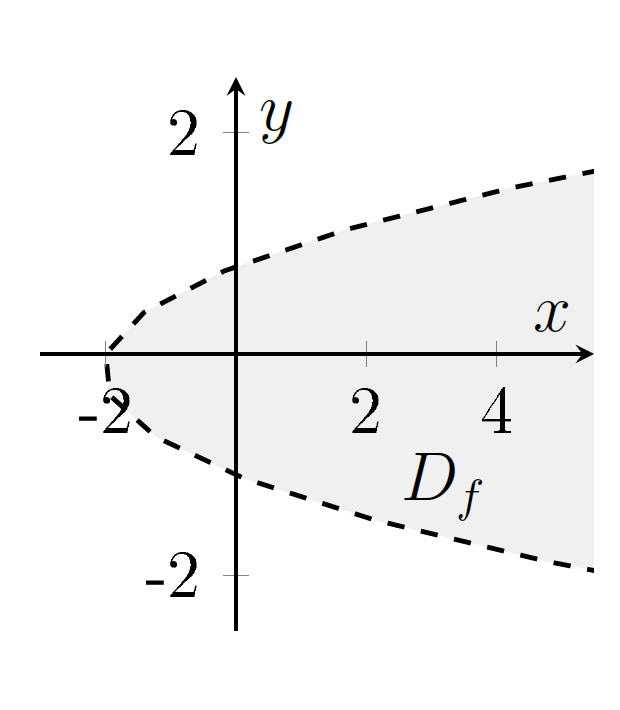
\includegraphics[scale=0.3]{pictures/BildA}
\item \text{} \\
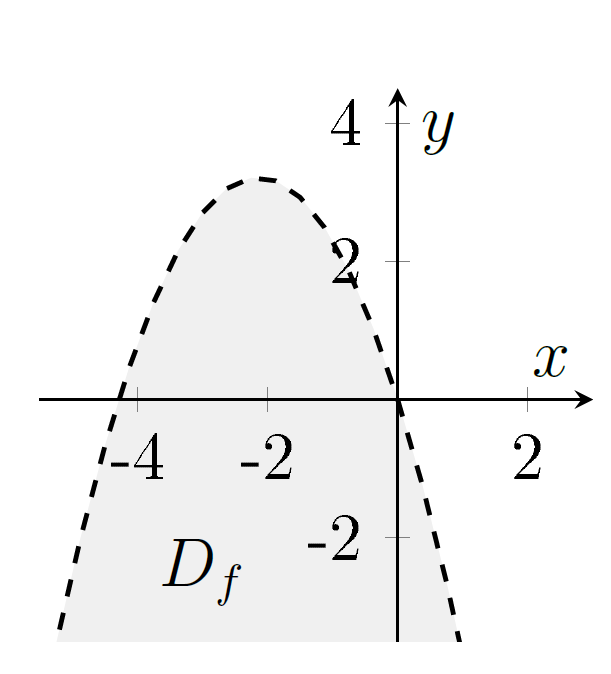
\includegraphics[scale=0.3]{pictures/BildB}
\item \text{} \\
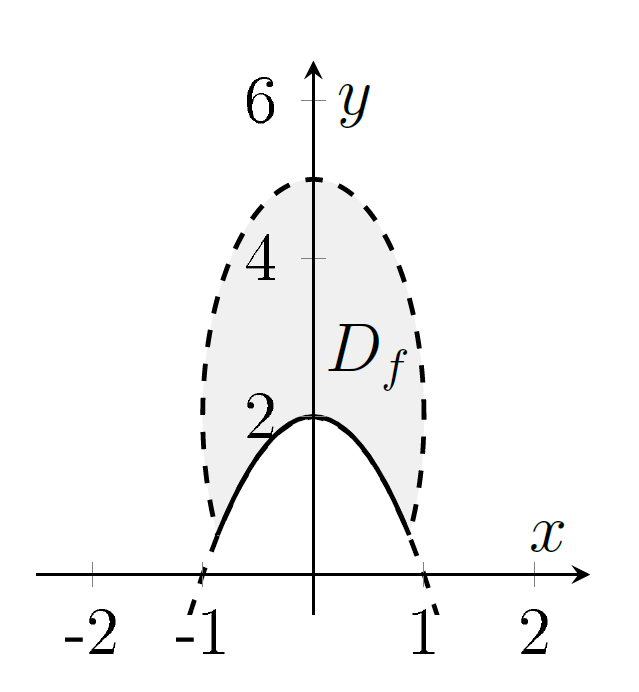
\includegraphics[scale=0.3]{pictures/BildC}
\item \text{} \\
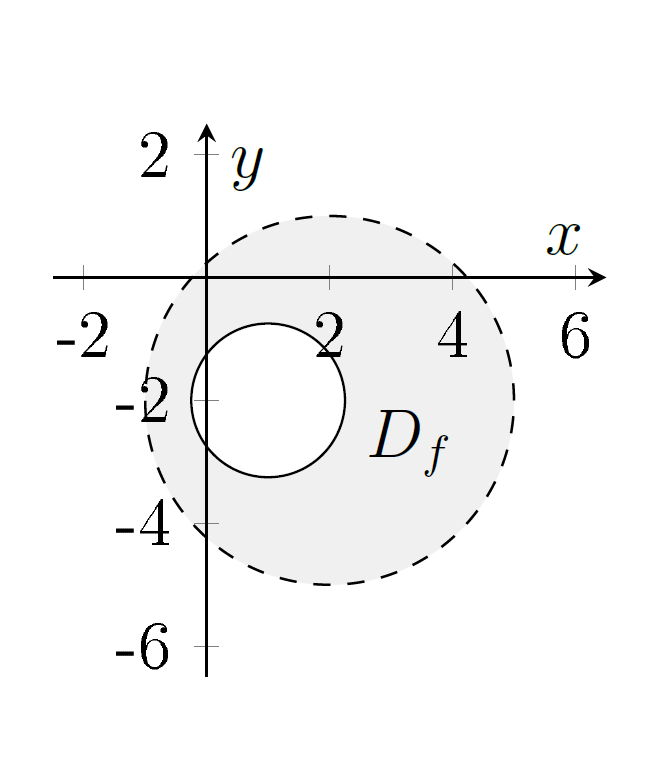
\includegraphics[scale=0.3]{pictures/BildD}
\end{enumerate}

\subsection*{\frage{5}{3}}
Eine homogene Funktion vom Grad 2 habe die partielle Elastizität 
$\varepsilon_{f,x}$ gleich $5x+1$.
Es folgt, dass
\renewcommand{\labelenumi}{(\alph{enumi})}
\begin{enumerate}
\item $\varepsilon_{f,y}(x,y) = -5x +1$.
\item $\varepsilon_{f,y}(x,y) = 5x +1$.
\item $\varepsilon_{f,y}(x,y) = -5x +2$.
\item $\varepsilon_{f,y}(x,y) = 5x +1$.
\end{enumerate}
 \ \\
\\
\subsection*{\frage{6}{3}}
Gegeben sei die Funktion $f$ definiert durch
\begin{align*}
f(x,y) = \sqrt[5]{x^{3.4}y^{0.6}}+ \sqrt{x^{0.8}y^{0.8}} 
+ \sqrt[3]{x^{1.6}y^{0.7}}
\end{align*}
wobei $x >0$ und $y> 0$.
\renewcommand{\labelenumi}{(\alph{enumi})}
\begin{enumerate}
\item $f$ ist homogen vom Grad $0.6$.
\item $f$ ist homogen vom Grad $0.7$.
\item $f$ ist homogen vom Grad $0.8$.
\item $f$ ist nicht homogen.
	
\end{enumerate}
\newpage
\subsection*{\frage{7}{3}}
Gegeben sei die Funktion $f$ definiert durch
\begin{align*}
f(x,y) = x^{3.1} \sqrt{y} + 6 y^{3.5} \sqrt{ 5 x^{0.2}}
		+ x^a y^{2a}
\end{align*}
wobei $x > 0 $, $ y >0 $ und $a \in \mathbb{R}$.\\
Für welchen Wert von $a$ ist $f$ homogen?
\renewcommand{\labelenumi}{(\alph{enumi})}
\begin{enumerate}
\item $a = 1$.
\item $a = 1.2$.
\item $a = 1.4$.
\item $f$ ist für kein $a \in \mathbb{R}$ homogen.
	
\end{enumerate}
\ \\
\\
\subsection*{\frage{8}{2}}
Die Funktion zweier reeller Variablen $f$ ist homogen vom Grad $3$ und die Funktion zweier reeller Variablen $g$ ist homogen vom Grad $2$.
Die Funktion $h$ ist definiert durch
$h(x,y) = f\left( (g(x,y))^2, (g(x,y))^2 \right)$.
Dann gilt
\renewcommand{\labelenumi}{(\alph{enumi})}
\begin{enumerate}
\item $\varepsilon_{h,x}(x,y) + \varepsilon_{h,y}(x,y) = 3$.
\item $\varepsilon_{h,x}(x,y) + \varepsilon_{h,y}(x,y) = 6$.
\item $\varepsilon_{h,x}(x,y) + \varepsilon_{h,y}(x,y) = 12$.
\item $\varepsilon_{h,x}(x,y) + \varepsilon_{h,y}(x,y) = 18$.
\end{enumerate}
